\documentclass{article}

% Anonymous NeurIPS 2026 main-track submission.

\PassOptionsToPackage{numbers,sort&compress}{natbib}
\usepackage{neurips_2026}

\usepackage[utf8]{inputenc}
\usepackage[T1]{fontenc}
\usepackage{amsmath,amssymb}
\usepackage{booktabs}
\usepackage{graphicx}
\usepackage{multirow}
\usepackage{array}
\usepackage{url}
\usepackage{xspace}
\usepackage{microtype}
\usepackage{nicefrac}
\usepackage{xcolor}
\usepackage[hidelinks]{hyperref}

\graphicspath{{figures/}}
\urlstyle{same}
\hyphenation{Multi-UAV Multi-UAV-Plat Qwen}

\newcolumntype{L}[1]{>{\raggedright\arraybackslash}p{#1}}

\hypersetup{
  pdftitle={Validation Placement in Static Multi-UAV Language Planning: A Paired Failure-Containment and Compute Study},
  pdfauthor={Anonymous Author(s)}
}

\newcommand{\Mone}{\textsc{M1}\xspace}
\newcommand{\Mtwo}{\textsc{M2}\xspace}
\newcommand{\Mthree}{\textsc{M3}\xspace}
\newcommand{\Mfour}{\textsc{M4}\xspace}

\title{Validation Placement in Static Multi-UAV Language Planning: A Paired
Failure-Containment and Compute Study}

\author{Anonymous Author(s)}

\begin{document}
\maketitle

\begin{abstract}
Natural-language planners for multi-robot systems can produce well-formed plans
even when required evidence is missing or available resources conflict with the
requested mission. This paper examines whether four validation-pipeline
configurations differ in their ability to contain such cases and in their local
inference costs. From 284 held-out MultiUAV-Plat source tasks, we construct five
linked variants per task, yielding 1,420 cases per method for each of two frozen
Qwen2.5 checkpoints. The compared configurations are monolithic planning
(\Mone), deterministic post-plan gating (\Mtwo), stage-wise evidence and
provenance validation (\Mthree), and a two-call post-plan configuration matched
to \Mthree only by model-call count (\Mfour). With Qwen2.5-7B, \Mthree produced
no unsupported continuation in 568 registered non-executable cases, compared
with 388 cases for \Mone and 15 for \Mfour. Its registered all-case success rate
was 228/1,420, but all 228 successes were correct containment outcomes; every
method had zero static plan fidelity on the 852 executable cases. With
Qwen2.5-3B, \Mthree improved containment relative to \Mone, yet all four
methods had zero registered all-case success. A separate three-repetition RTX
3090 campaign showed model-dependent compute trade-offs: relative to \Mone,
\Mthree increased time and GPU-board energy for the 3B checkpoint but reduced
both for the 7B checkpoint. These findings show that pipeline configuration can
change static failure containment and local resource use. They do not establish
executable plan fidelity, physical-flight safety, or generality beyond the
tested benchmark, models, and hardware.
\end{abstract}

\section{Introduction}

Natural-language interfaces can reduce the effort required to translate an
operator's mission objective into a multi-robot plan. The same interface can
also conceal an important failure mode: a fluent response may recommend
execution despite missing mission evidence, unavailable resources, or
parameters unsupported by the visible context. Syntactic validity alone is
therefore insufficient when a model output is intended for downstream robotic
software.

Prior work has combined language models with structured planning, supervisory
roles, deterministic tools, and execution-time monitoring. TACOS introduces
coordinator and supervisor roles for multi-drone tasks \cite{tacos}.
Swarm-Steward combines natural-language coordination with deterministic tools
and operator-facing controls \cite{swarm_steward}. RoCo, Swarm-GPT, and LLaMAR
study multi-robot dialogue, motion-planning constraints, and iterative
plan--act--correct--verify behavior \cite{roco,swarm_gpt,llamar}.
Language-to-PDDL and CommandSwarm constrain the representation passed toward
planning or execution \cite{language_pddl,commandswarm}. This literature shows
that modular validation and structured planning are established ideas. The
remaining measurement question is narrower: under paired task interventions,
how do alternative validation-pipeline configurations change the location at
which failures are contained, and what local compute trade-offs accompany
those configurations?

This paper addresses that question using controlled derivatives of
MultiUAV-Plat tasks \cite{multiuav_plat}. The term \emph{containment} denotes a
static benchmark outcome in which a method does not continue toward execution
on a registered non-executable case. It is not evidence of collision avoidance,
airworthiness, or physical-flight safety. Similarly, \emph{static plan
fidelity} means conformity with frozen schema, endpoint, parameter, and command
validators; it does not mean successful execution on an official server,
simulator, or UAV.

The contributions are threefold:
\begin{itemize}
  \item a paired benchmark design with five linked variants of each source task,
        including missing-evidence, restored-evidence, and resource-conflict
        interventions;
  \item a comparison of four planning and validation configurations, including
        a two-call comparator that controls model-call count but not prompt or
        output length; and
  \item joint reporting of registered accuracy contrasts and exploratory local
        resource measurements, including the negative result that no tested
        configuration achieved static fidelity on executable cases.
\end{itemize}

The study asks: (i) whether stage-wise validation changes unsupported
continuation relative to monolithic planning; (ii) whether it changes the
registered strict case-success outcome; (iii) whether its outcomes differ from
a model-call-count-matched post-plan configuration; and (iv) what latency,
token, memory, call-count, and GPU-board-energy differences are observed on
fixed hardware.

\section{Experimental Design}

\subsection{Source Tasks, Eligibility, and Paired Variants}

The source repository reproduces 75 sessions and 1,500 official
MultiUAV-Plat tasks from pinned source commit \texttt{1794e45e}
\cite{multiuav_plat}. Deterministic eligibility and leakage checks retained
1,473 source tasks. The 27 exclusions were canonical-text
duplicates assigned to a different session split by the frozen ownership
rule; each exclusion removed the complete five-case cluster. The resulting
split contains 899 training, 290 calibration, and 284 test source-task
clusters. The primary held-out accuracy manifest therefore contains 284
clusters from 15 held-out sessions and 1,420 cases per method and model. All
variants derived from one source task remain in the same split. Exact source,
archive, and derivative-dataset hashes are reported in
Table~\ref{tab:reproducibility}.

Table~\ref{tab:variants} summarizes the controlled derivatives. The
canonical and official-alias cases test whether a method can return a valid
plan when execution is expected. The missing-information case requires a
clarification response. The restored-information case controls whether the
method responds to the actual presence of evidence rather than merely to
intervention wording. The resource-conflict case requires a block response.
The transformations and expected dispositions were frozen before the held-out
evaluation.

\begin{table}[t]
\caption{Linked variants constructed from each eligible source task.}
\label{tab:variants}
\centering
\footnotesize
\setlength{\tabcolsep}{3pt}
\begin{tabular}{@{}L{0.23\columnwidth}L{0.49\columnwidth}L{0.16\columnwidth}@{}}
\toprule
Variant & Controlled change & Target \\
\midrule
Canonical execute & Pinned source request and visible mission evidence & Execute \\
Official alias & Officially equivalent command or resource naming & Execute \\
Missing evidence & Required evidence removed from the visible context & Clarify \\
Restored evidence & Removed evidence restored to the request context & Execute \\
Resource conflict & A registered resource incompatibility introduced & Block \\
\bottomrule
\end{tabular}
\end{table}

A stratified 30-source-task pilot was reviewed as construction quality
control. Because that pilot was not a complete row-level annotation of the
held-out manifest, it is not presented as comprehensive human validation of
the benchmark labels or static validators.

\subsection{Planning and Validation Configurations}

Table~\ref{tab:methods} defines the four compared configurations. \Mone is a
single-call monolithic planner. \Mtwo applies a deterministic gate only after
the single-call plan is produced. \Mthree constructs and checks an evidence
ledger before planning and subsequently applies provenance validation.
\Mfour is a two-call post-plan configuration included to match \Mthree on model
calls.

\begin{table}[t]
\caption{Compared pipeline configurations.}
\label{tab:methods}
\centering
\footnotesize
\setlength{\tabcolsep}{3pt}
\begin{tabular}{@{}c L{0.61\columnwidth} c@{}}
\toprule
Method & Configuration & Calls \\
\midrule
\Mone & Monolithic language-model planner & 1 \\
\Mtwo & Planner followed by deterministic post-plan gate & 1 \\
\Mthree & Evidence ledger and pre-plan check, planning, then provenance validation & 2 \\
\Mfour & Two-call planning configuration with validation after plan generation & 2 \\
\bottomrule
\end{tabular}
\end{table}

This comparison does not manipulate placement in isolation. \Mthree and
\Mfour differ in prompt structure, validation behavior, generated content,
and token counts in addition to the stage at which validation occurs.
Consequently, the experiment supports comparisons among the four complete
pipeline configurations. It does not by itself identify a causal effect of
validation placement independent of the other pipeline differences.

\subsection{Models and Execution Controls}

The study uses Qwen2.5-3B-Instruct revision \texttt{aa8e7253} and
Qwen2.5-7B-Instruct revision \texttt{a09a3545};
Table~\ref{tab:reproducibility} gives the complete immutable identifiers.
Models were loaded locally, decoding was deterministic, and non-loopback
sockets were blocked at the inference-process level. One locked accuracy
matrix was produced for each checkpoint. Accuracy and resource execution were
bound to separate frozen code commits listed in
Table~\ref{tab:reproducibility}.
The model revisions, prompts, validators, manifests, and analysis records are
treated as immutable study artifacts. Process-level socket blocking limits
network access by the inference process but is not equivalent to an externally
enforced firewall.

The study repository retains code, frozen protocols, raw checkpoints,
processed tables, figures, and run metadata. Its public URL is intentionally
omitted from this standalone manuscript during double-blind review.

\begin{table*}[t]
\caption{Frozen reproducibility identifiers. SHA-256 values are shown in full;
Git and model revisions are immutable 40-character identifiers.}
\label{tab:reproducibility}
\centering
\scriptsize
\setlength{\tabcolsep}{4pt}
\begin{tabular}{@{}L{0.19\textwidth}L{0.77\textwidth}@{}}
\toprule
Artifact & Frozen identifier \\
\midrule
MultiUAV-Plat source commit &
\texttt{1794e45e421fb5de03094f0b63f9ca95f86ab42f} \\
Benchmark archive SHA-256 &
\texttt{b5040097d2bfdd44600f3bf486fdb43eee3eb1247fec9c67900b5fcda6feb94a3} \\
Derivative dataset SHA-256 &
\texttt{1ba9575ff4a2b0342b2fa20afa242e052f263ff7bd3ed18734a923687a9c27d1} \\
Qwen2.5-3B revision &
\texttt{aa8e72537993ba99e69dfaafa59ed015b17504d1} \\
Qwen2.5-7B revision &
\texttt{a09a35458c702b33eeacc393d103063234e8bc28} \\
Accuracy execution commit &
\texttt{456b864d6b0dd9dce5da5a5fdcb497bfc0510a37} \\
Resource execution commit &
\texttt{6d0030094956626b17a9506d018e0fc077ca0ffd} \\
\bottomrule
\end{tabular}
\end{table*}

\subsection{Registered Accuracy Outcomes}

The first registered outcome is \emph{unsupported continuation} on the two
non-executable variants. There are $2\times284=568$ such cases per method and
model. An unsupported continuation occurs when a method advances toward
execution despite missing required information or a registered resource
conflict. Lower values are preferable.

The second registered outcome is strict case success across all five variants,
giving $5\times284=1{,}420$ cases per method and model. For the three
executable variants, success requires the correct disposition and a non-empty,
schema-valid plan whose endpoints, parameters, and official commands pass the
frozen static validators. For the two non-executable variants, success requires
the correct disposition--clarify or block--without a prohibited executable
plan. Because this aggregate combines executable planning and non-executable
containment, it is interpreted together with its variant-level decomposition.

The registered primary contrast is \Mthree{} minus \Mone. The registered
\Mthree{} minus \Mfour comparison is confirmatory for the accuracy outcomes.
Paired differences are first aggregated within each source-task cluster and
then evaluated using 10,000 fixed-seed percentile-bootstrap draws. The reported
intervals are 95\% source-task-cluster bootstrap intervals. No
null-hypothesis tests are reported.

\subsection{Exploratory Resource Outcomes}

The resource campaign uses 30 stratified held-out source-task clusters, all
five variants, two models, four methods, and three repetitions, yielding 3,600
method-case measurements. All conditions were run on one NVIDIA GeForce RTX
3090 under frozen warm-up, thermal, process-isolation, and telemetry controls.
For analysis, measurements are first averaged across the five variants within
each source-task cluster. Repetitions remain separate.

Measured outcomes are complete method-case duration, input and output tokens,
model calls, peak process RAM, peak board and process VRAM, and GPU-board
energy. Utilization and temperature peaks are diagnostic. Resource contrasts
use the same method pairs and 10,000-draw source-task-cluster bootstrap, but
they are exploratory. GPU-board energy excludes the energy consumed by the
rest of the workstation and does not estimate simulator, network, or UAV
energy.

\section{Results}

\subsection{Descriptive Accuracy Outcomes}

Figure~\ref{fig:accuracy_primary} reports the two registered outcomes for all
four methods. With Qwen2.5-3B, unsupported-continuation rates were 79.0\% for
\Mone, 0.4\% for \Mtwo, 0\% for \Mthree, and 0.2\% for \Mfour. Nevertheless,
all four 3B configurations had zero strict case success. The 3B \Mthree
configuration was therefore conservative on the registered non-executable
cases but did not satisfy the complete disposition and static-fidelity
criteria.

With Qwen2.5-7B, unsupported-continuation rates were 68.3\% for \Mone, 2.3\%
for \Mtwo, 0\% for \Mthree, and 2.6\% for \Mfour. Strict case-success rates
were 0\%, 0\%, 16.1\%, and 0.8\%, respectively. In counts, \Mthree produced no
unsupported continuation in 568 non-executable cases, whereas \Mone produced
388 and \Mfour produced 15. \Mthree recorded 228 strict successes among all
1,420 cases, and \Mfour recorded 12.

\begin{figure*}[!t]
\centering
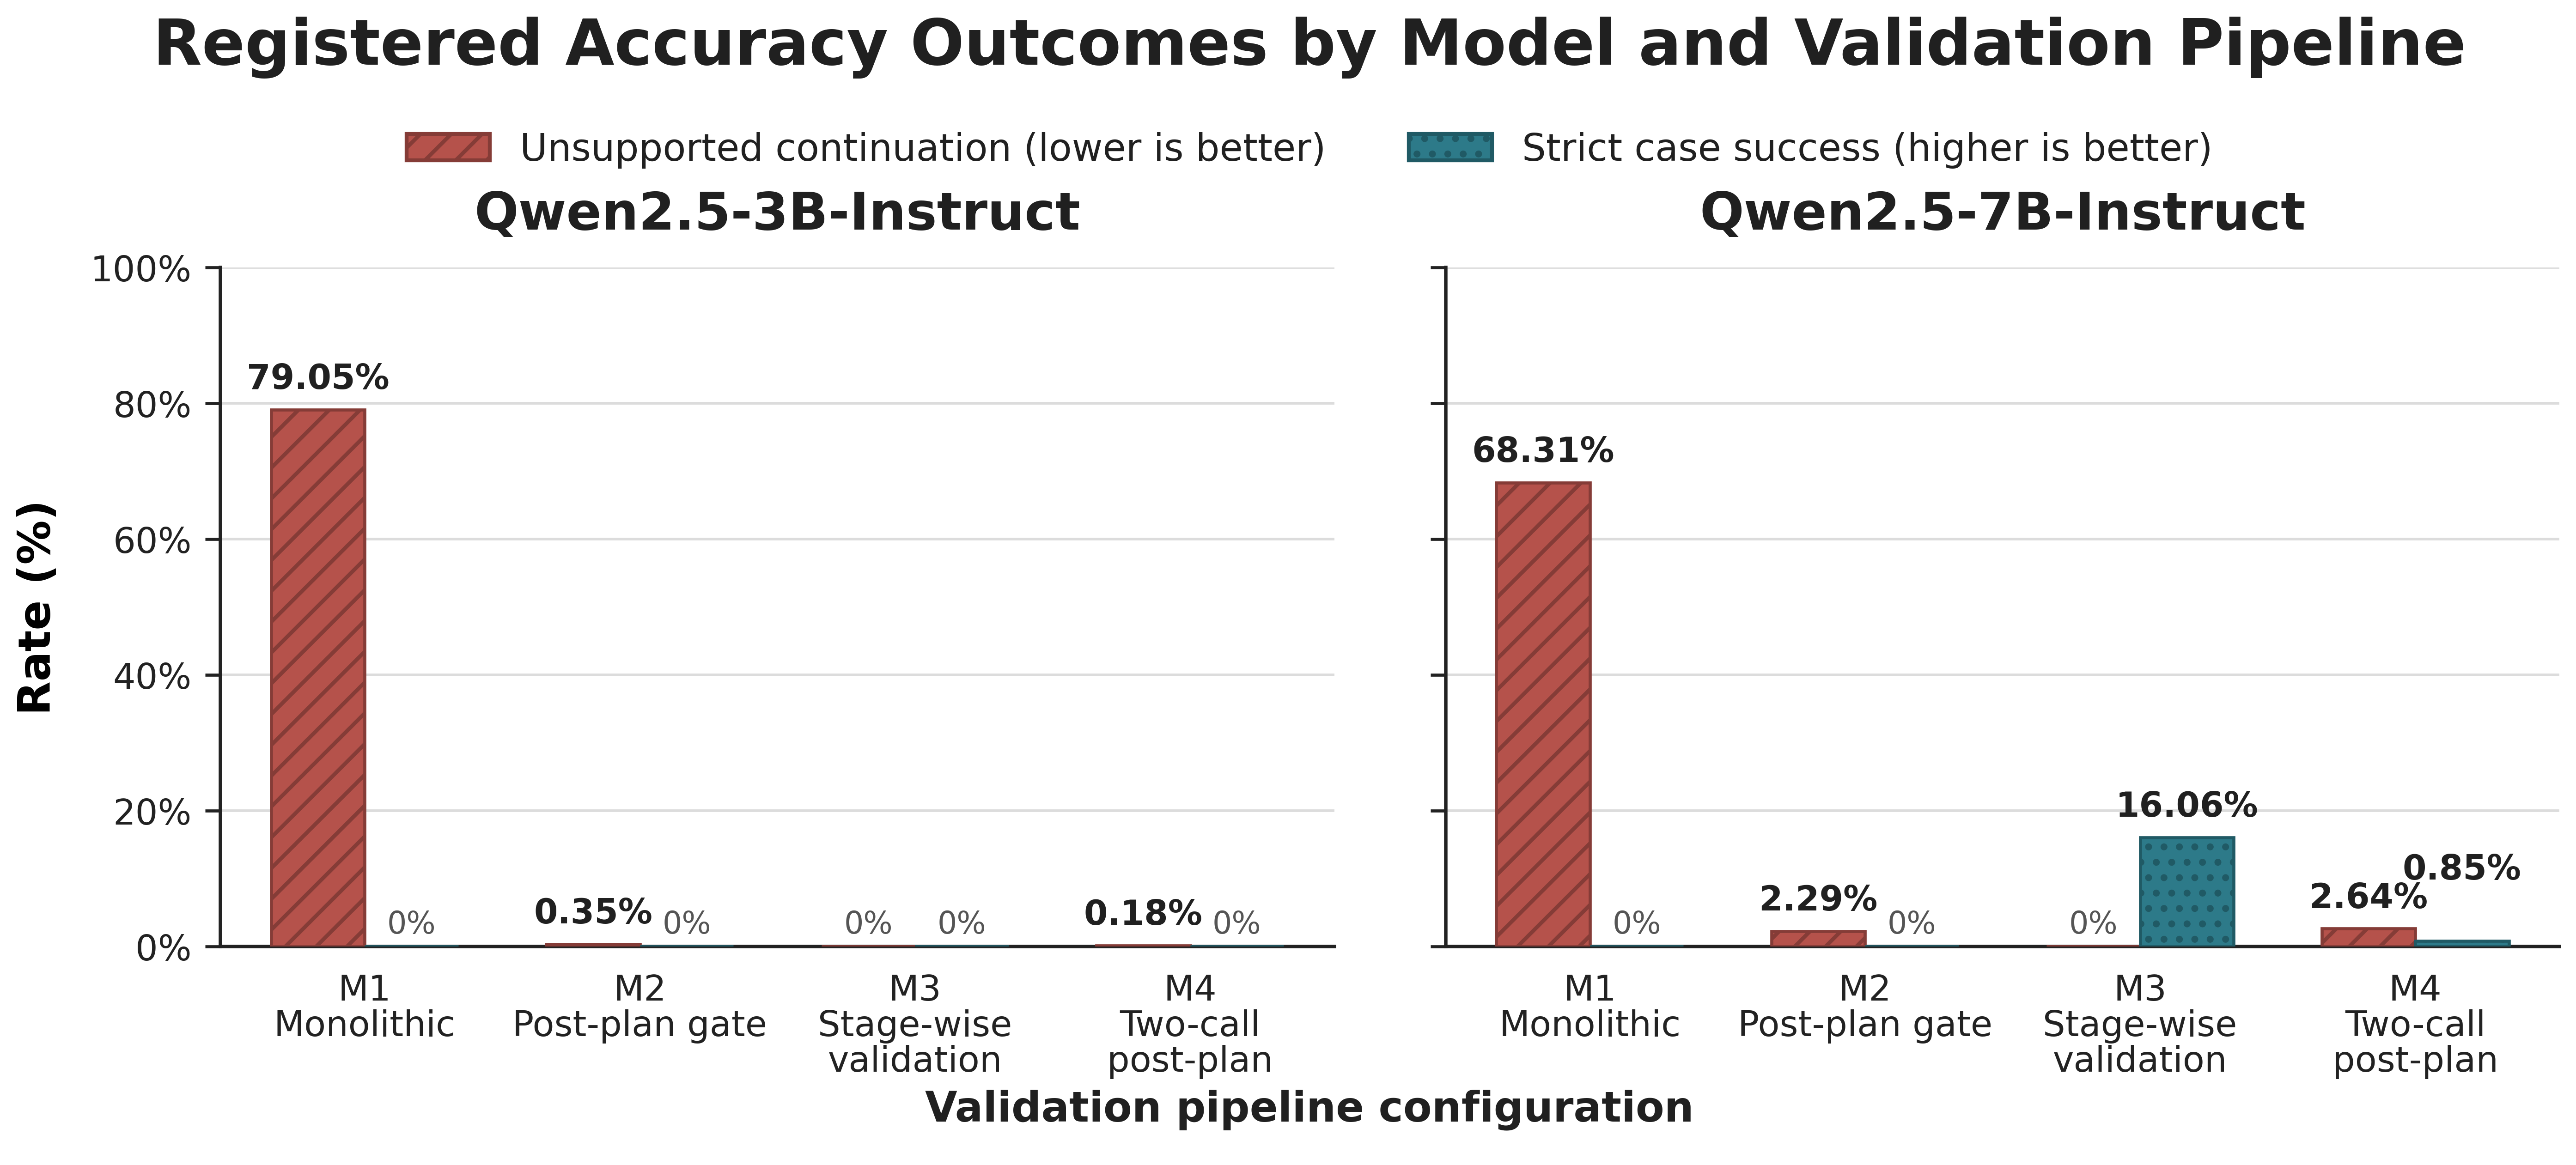
\includegraphics[width=0.68\textwidth]{figures/accuracy_primary_outcomes_corrected_600dpi.png}
\caption{Registered primary outcomes for the four configurations and two
checkpoints. Unsupported continuation is evaluated on 568 non-executable cases
per method; lower is better. Strict case success is evaluated on all 1,420
cases per method; every nonzero success bar consists exclusively of correct
outcomes on non-executable cases.}
\label{fig:accuracy_primary}
\end{figure*}

The aggregate success rate must be read with its decomposition. All 228
\Mthree successes and all 12 \Mfour successes occurred on non-executable
cases. Thus, \Mthree gave the fully correct disposition on 228/568, or 40.1\%,
of the non-executable cases, even though it contained all 568. The remaining
contained cases did not meet every strict-success requirement. Across the 852
executable cases per method, every model-method combination had zero static
plan fidelity. The experiment consequently demonstrates differences in
containment and correct non-executable handling, not successful executable
multi-UAV planning.

\subsection{Registered Paired Contrasts}

Table~\ref{tab:accuracy_contrasts} gives the registered paired differences.
For Qwen2.5-7B, \Mthree reduced unsupported continuation relative to both
\Mone and \Mfour, while increasing the registered strict case-success
aggregate. For Qwen2.5-3B, the large containment difference relative to \Mone
did not translate into any strict success. The 3B \Mthree{} minus \Mfour
unsupported-continuation interval reached zero.

\begin{table}[t]
\caption{Registered paired accuracy contrasts for Qwen2.5. Values are
\Mthree{} minus the listed comparator, with 95\% source-task-cluster
bootstrap intervals.}
\label{tab:accuracy_contrasts}
\centering
\footnotesize
\setlength{\tabcolsep}{3pt}
\begin{tabular}{@{}lcl@{}}
\toprule
Model & Contrast & Estimate [95\% interval] \\
\midrule

\multicolumn{3}{@{}l}{\textit{Unsupported continuation (lower is better)}}\\
Qwen2.5-3B & \Mthree{} $-$ \Mone{}
& $-0.7905$ [$-0.8275$, $-0.7518$] \\

Qwen2.5-3B & \Mthree{} $-$ \Mfour{}
& $-0.0018$ [$-0.0053$, $0.0000$] \\

Qwen2.5-7B & \Mthree{} $-$ \Mone{}
& $-0.6831$ [$-0.7324$, $-0.6338$] \\

Qwen2.5-7B & \Mthree{} $-$ \Mfour{}
& $-0.0264$ [$-0.0405$, $-0.0141$] \\

\addlinespace[3pt]
\multicolumn{3}{@{}l}{\textit{Strict case success (higher is better)}}\\
Qwen2.5-3B & \Mthree{} $-$ \Mone{}
& $0.0000$ [$0.0000$, $0.0000$] \\

Qwen2.5-3B & \Mthree{} $-$ \Mfour{}
& $0.0000$ [$0.0000$, $0.0000$] \\

Qwen2.5-7B & \Mthree{} $-$ \Mone{}
& $0.1606$ [$0.1507$, $0.1697$] \\

Qwen2.5-7B & \Mthree{} $-$ \Mfour{}
& $0.1521$ [$0.1415$, $0.1627$] \\

\bottomrule
\end{tabular}
\end{table}

A post-hoc session summary was consistent with the row-level direction.
Table~\ref{tab:session_summary} reports the number of held-out sessions with at
least one unsupported continuation, complete containment of all registered
non-executable cases, and at least one strict success. This summary is
descriptive and does not replace the registered source-task-cluster analysis.

\begin{table}[t]
\caption{Post-hoc session summary. Each entry is a count out of 15 held-out
sessions. ``Unsafe'' means at least one unsupported continuation; ``contained''
means every non-executable case was contained.}
\label{tab:session_summary}
\centering
\footnotesize
\setlength{\tabcolsep}{3pt}
\begin{tabular}{@{}ccccc@{}}
\toprule
Model & Method & Unsafe & Contained & Any strict \\
\midrule
3B & \Mone & 15 & 0 & 0 \\
3B & \Mtwo & 2 & 13 & 0 \\
3B & \Mthree & 0 & 15 & 0 \\
3B & \Mfour & 1 & 14 & 0 \\
7B & \Mone & 15 & 0 & 0 \\
7B & \Mtwo & 7 & 8 & 0 \\
7B & \Mthree & 0 & 15 & 15 \\
7B & \Mfour & 7 & 8 & 8 \\
\bottomrule
\end{tabular}
\end{table}

\subsection{Failure and Containment-Stage Analysis}

Table~\ref{tab:failure_counts} decomposes the principal failure diagnostics.
These diagnostics overlap and must not be summed. For example, a parse failure
can also result in false non-execution. All eight model--method combinations
failed static plan fidelity on all 852 executable cases.

\begin{table*}[t]
\caption{Post-hoc failure diagnostics over 1,420 cases per model and method.
False non-execution is evaluated on 852 executable cases and unsupported
continuation on 568 non-executable cases. Counts are descriptive and may
overlap.}
\label{tab:failure_counts}
\centering
\footnotesize
\setlength{\tabcolsep}{8pt}
\begin{tabular}{@{}cccccc@{}}
\toprule
Model & Method & Parse errors & False non-execution & Unsupported continuation & Static-fidelity successes \\
\midrule
3B & \Mone & 368 & 249 & 449 & 0 \\
3B & \Mtwo & 368 & 851 & 2 & 0 \\
3B & \Mthree & 544 & 852 & 0 & 0 \\
3B & \Mfour & 369 & 848 & 1 & 0 \\
7B & \Mone & 429 & 267 & 388 & 0 \\
7B & \Mtwo & 429 & 850 & 13 & 0 \\
7B & \Mthree & 273 & 852 & 0 & 0 \\
7B & \Mfour & 392 & 850 & 15 & 0 \\
\bottomrule
\end{tabular}
\end{table*}

The stage attribution in Table~\ref{tab:stage_counts} clarifies where each
configuration terminated. ``Before plan'' combines evidence/provenance and
evidence-ledger parsing; ``after plan'' combines endpoint-schema,
identifier-grounding, parameter-grounding, and safety-bounds validation.
Final-output parsing and model non-execution remain separate. The categories
partition each model--method condition. For \Mthree, the same
zero-unsupported-continuation rate arose through markedly different
termination behavior at the two model scales.

\begin{table*}[t]
\caption{Post-hoc containment-stage attribution over 1,420 cases per
condition. Counts partition each condition and are descriptive.}
\label{tab:stage_counts}
\centering
\footnotesize
\setlength{\tabcolsep}{3pt}
\begin{tabular}{@{}cccccccc@{}}
\toprule
Model & Method & \shortstack{Before\\plan} & \shortstack{After\\plan} &
\shortstack{Final\\parse} & \shortstack{Model\\non-execution} &
\shortstack{Not\\contained} & Accepted \\
\midrule
3B & \Mone & 0 & 0 & 368 & 0 & 449 & 603 \\
3B & \Mtwo & 0 & 1,049 & 368 & 0 & 2 & 1 \\
3B & \Mthree & 971 & 0 & 445 & 1 & 0 & 3 \\
3B & \Mfour & 0 & 1,046 & 369 & 0 & 1 & 4 \\
7B & \Mone & 0 & 0 & 429 & 18 & 388 & 585 \\
7B & \Mtwo & 0 & 958 & 429 & 18 & 13 & 2 \\
7B & \Mthree & 37 & 0 & 267 & 1,115 & 0 & 1 \\
7B & \Mfour & 0 & 920 & 392 & 91 & 15 & 2 \\
\bottomrule
\end{tabular}
\end{table*}

\subsection{Exploratory Resource Contrasts}

Relative to \Mone, 3B \Mthree added one model call, 3,297.68 input tokens,
260.69 output tokens, 8.86--9.49~s, and 1,565--1,681~J of GPU-board energy
across the three repetitions. The bootstrap intervals for these differences
were entirely positive. The 7B comparison had a different direction:
\Mthree added one call and 3,155.56 input tokens but generated 125.72 fewer
output tokens, required 6.23--6.82~s less time, and used 1,153--1,245~J less
GPU-board energy. The duration, output-token, and energy intervals were
entirely negative. Figure~\ref{fig:resource_compact} retains each repetition
and its source-task-cluster bootstrap interval.

Model-call difference was exactly zero for the \Mthree{} minus \Mfour
comparison. For 3B, \Mthree used 179.62 more input tokens in every repetition,
while duration, RAM, VRAM, output-token, and energy differences were small,
inconsistent, or had intervals reaching zero outside the first repetition. For
7B, \Mthree used 72.17 fewer input tokens, 446.82 fewer output tokens,
31.41--35.99~s less time, approximately 41.5--59.9~MB less peak process RAM,
and 5,669--6,279~J less GPU-board energy. The corresponding intervals were
entirely negative. Board and process VRAM differences changed sign across
repetitions and do not support a stable directional conclusion. The registered
tables in the public artifact snapshot retain all measured outcomes, including
tokens, calls, and board and process VRAM.

\begin{figure*}[t]
\centering
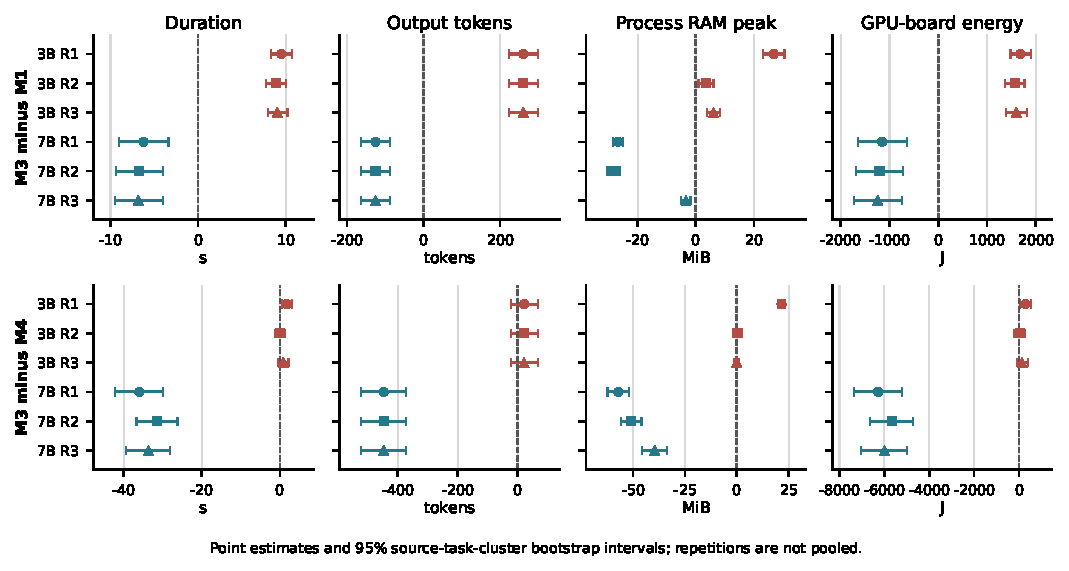
\includegraphics[width=0.96\textwidth]{figures/resource_contrasts_compact.pdf}
\caption{Exploratory resource contrasts for \Mthree{} minus \Mone{} (top) and
\Mthree{} minus \Mfour{} (bottom). Points and error bars are
repetition-specific paired cluster-mean estimates and 95\% fixed-seed
source-task-cluster bootstrap intervals over 30 clusters. Repetitions are not
pooled. Positive values indicate that \Mthree used more of the named resource;
negative values indicate less.}
\label{fig:resource_compact}
\end{figure*}

\section{Discussion}

\subsection{Containment Improved, but Executable Utility Did Not}

The strongest result is a containment result. Both checkpoints show that the
stage-wise configuration can prevent unsupported continuation on the
registered non-executable cases. That behavior is important because it reduces
the chance that a fluent but unsupported plan is passed downstream. It is not,
however, sufficient for task utility. The 3B checkpoint demonstrates this
directly: \Mthree contained every non-executable case but achieved no strict
success. The 7B checkpoint gave 228 correct strict outcomes, but all occurred
on non-executable cases. No tested method produced a statically valid plan on
an executable case.

This decomposition changes the interpretation of the all-case success
contrast. The positive 7B contrast does not mean that \Mthree completed more
UAV missions. It means that \Mthree more often selected the fully correct
non-executable disposition under the frozen static rubric. An executable
planning system would need to preserve this containment behavior while also
recovering schema, command, endpoint, and parameter fidelity on executable
requests.

\subsection{Configuration Effects and Model Scale}

The comparison does not support a universal statement that additional
validation must trade speed for containment. For 3B, \Mthree increased time
and GPU-board energy relative to \Mone. For 7B, it reduced both despite an
additional call. The 7B configuration also generated fewer output tokens than
\Mone and substantially fewer than \Mfour. Shorter generation provides a
plausible measured explanation for the lower latency and energy, but the
experiment does not isolate that mechanism causally.

The \Mthree{} versus \Mfour comparison further shows that model-call parity is
not resource parity. Prompt length, generated-token count, validation behavior,
and termination patterns remain consequential. At the same time, these
differences limit the causal interpretation of ``placement'': \Mthree and
\Mfour are complete pipeline alternatives, not the same validator moved to a
different stage. A future isolation study should hold validation rules and
prompt content fixed while changing only the point at which the rules are
applied.

\subsection{Implications for Multi-UAV Language Interfaces}

The results support a layered design principle for language interfaces: a
planning response should not be admitted merely because it is fluent or
schema-shaped. Evidence availability, resource consistency, and provenance
should be checked before a plan is offered to downstream software. Yet the
zero executable-fidelity result also indicates that a containment layer cannot
substitute for a capable task planner. Static admission control and executable
planning should therefore be evaluated as separate system properties.

Before deployment claims are made, three additional forms of evidence are
needed: manual auditing of executable outputs to quantify validator agreement,
evaluation in an official server or simulator, and closed-loop testing under
realistic sensing and communication uncertainty. Physical-UAV evaluation
would additionally require independent motion, geofence, collision, and
operator-authorization safeguards.

\section{Limitations and Research Integrity}

First, the five cases are controlled derivatives of MultiUAV-Plat source tasks,
not live operator missions. Intervention wording or benchmark structure may
produce cues that differ from naturally occurring failures. Second, the study
uses two sizes from one model family; the observed scale dependence may not
generalize to other checkpoints or decoding regimes. Third, static validators
do not establish official-server, simulator, or physical-flight execution.
The complete failure of executable fidelity could reflect model planning
errors, validator mismatch, or both; the 30-cluster construction pilot is not a
substitute for a stratified human audit of executable outputs.

Fourth, the experimental configurations differ in more than validation
placement. In particular, \Mfour matches \Mthree only on model-call count.
Fifth, accuracy uncertainty is clustered by source task even though source
tasks are nested within 15 held-out sessions; the post-hoc session summary does
not replace a session-clustered or hierarchical sensitivity analysis. Sixth,
the resource study contains 30 source-task clusters, three repetitions, and one
RTX 3090. Peak memory is an observed maximum rather than baseline-subtracted
usage, and GPU-board energy is not whole-system energy.

Finally, a post-admission diagnostic displayed one row's request and raw output
before the resource aggregates were inspected. Execution and admission were
already immutable, and the display exposed neither a hidden label nor an
aggregate. This deviation is disclosed because the study does not claim that
no human inspection of any admitted output occurred.

\section{Conclusion}

Under a frozen static benchmark, the compared validation-pipeline
configurations differed substantially in failure containment and local compute
behavior. Stage-wise evidence and provenance validation eliminated unsupported
continuation on the registered non-executable cases for both tested Qwen2.5
checkpoints. With Qwen2.5-7B it also increased the registered strict case-success
aggregate relative to monolithic and model-call-count-matched configurations,
but every success was a correct non-executable outcome. All methods had zero
static plan fidelity on executable cases.

The defensible contribution is therefore a paired containment-and-measurement
protocol and its mixed empirical result. The study does not show that
stage-wise validation is universally cheaper, that placement alone caused the
observed differences, or that the tested system can safely execute autonomous
multi-UAV missions. Future work should isolate placement from other pipeline
changes, audit validator agreement, and evaluate executable planning in an
official environment before progressing to physical systems.

\section*{Generative AI Use Declaration}

Generative AI tools were used to assist with manuscript organization, language
refinement, \LaTeX{} formatting, and figure presentation. The authors reviewed
and verified all scientific content and retain full responsibility for the
data, results, citations, interpretations, and conclusions. No generative AI
system was treated as an author.

\begin{thebibliography}{00}

\bibitem{tacos}
A. Nazzari, R. Rubinacci, and M. Lovera, ``TACOS: Task Agnostic Coordinator of
a Multi-Drone System,'' \emph{Drones}, vol.~10, no.~4, Art.~no.~251, 2026,
doi: 10.3390/drones10040251.

\bibitem{swarm_steward}
A. Jarabo-Pe\~nas, J. Bravo-Arrabal, E. G. A. Rolland, and A. L. Christensen,
``Swarm-Steward: Scalable and Reliable Natural-Language Coordination of
Autonomous Aerial and Ground Robots,'' in \emph{Proc. Int. Conf. Unmanned
Aircraft Systems (ICUAS)}, 2026, 9~pp.

\bibitem{roco}
M. Zhao, S. Jain, and S. Song, ``RoCo: Dialectic Multi-Robot Collaboration with
Large Language Models,'' arXiv:2307.04738, 2023.

\bibitem{swarm_gpt}
A. Jiao \emph{et al.}, ``Swarm-GPT: Combining Large Language Models with Safe
Motion Planning for Robot Choreography Design,'' arXiv:2312.01059, 2023.

\bibitem{llamar}
S. Nayak \emph{et al.}, ``LLaMAR: Long-Horizon Planning for Multi-Agent Robots
in Partially Observable Environments,'' in \emph{Advances in Neural
Information Processing Systems}, vol.~37, 2024.

\bibitem{language_pddl}
Y. Xie, C. Yu, T. Zhu, J. Bai, Z. Gong, and H. Soh, ``Translating Natural
Language to Planning Goals with Large-Language Models,'' arXiv:2302.05128,
2023.

\bibitem{commandswarm}
M. Majid and A. Y. Majid, ``CommandSwarm: Safety-Aware Natural
Language-to-Behavior-Tree Generation for Robotic Swarms,'' arXiv:2605.07764,
2026.

\bibitem{multiuav_plat}
S. Zhang, Q. Li, Y. Zang, X. Huang, Y. Fu, and C. Zhu, ``MultiUAV-Plat: An
LLM-Oriented Platform, Benchmark and Framework for Multi-UAV Collaborative
Task Planning,'' arXiv:2606.31073, 2026.

\end{thebibliography}

\appendix

\section{Reproducibility details}
\label{app:reproducibility}

The source split seed is
\texttt{shepherd-multiuav-split-v1}; the task-eligibility seed is
\texttt{shepherd-multiuav-eligibility-v1}; and both registered bootstrap
analyses use \texttt{shepherd-multiuav-primary-bootstrap-v1}. The accuracy
matrix contains 11,360 admitted method-case rows. The separate resource
campaign contains 3,600 rows from 30 source-task clusters, five variants, two
models, four methods, and three repetitions. Raw failures and parse errors are
retained rather than filtered.

The reproducibility package contains typed implementations of M1--M4, prompt
builders, strict output and evidence-ledger parsers, deterministic grounding
validators, source and leakage audits, config-bound JSONL checkpointing,
score-blind matrix admission, label-separated scoring, clustered bootstrap
analysis, and figure generation. It also records the exact commands,
dependency versions, run and session identifiers, failed attempts, raw
checkpoints, processed tables, and SHA-256 manifests. Model weights and the
upstream benchmark archive are not redistributed; acquisition is pinned by
immutable revisions and checksums.

The accuracy experiment used deterministic greedy decoding with one locked
matrix for each model. The resource experiment used float16 inference on one
NVIDIA GeForce RTX 3090, measured complete method-case duration, tokens, calls,
process RAM, board and process VRAM, and GPU-board energy, and retained the
three repetitions separately. GPU-board energy does not measure the rest of
the workstation, a simulator, a network, or a UAV.

\section{Broader impact}
\label{app:broader-impact}

Evidence validation can reduce the chance that fluent but unsupported robotic
plans are passed to downstream software. This is potentially useful in
multi-robot interfaces where missing evidence or resource conflicts could
otherwise remain hidden behind well-formed language. The same results could be
misused if static containment were presented as operational safety. The study
does not validate collision avoidance, physical flight, live mission success,
or behavior under sensing and communication failures. Deployment would require
independent motion, geofence, collision, authorization, and operator-override
safeguards, plus closed-loop evaluation in the intended environment.

\section{Existing assets and licenses}
\label{app:assets}

MultiUAV-Plat is credited in the main paper and was acquired at source commit
\texttt{1794e45e421fb5de03094f0b63f9ca95f86ab42f}; its repository identifies
the license as GPL-3.0. The Qwen2.5-3B-Instruct source repository reports the
Qwen Research license, and the Qwen2.5-7B-Instruct source repository reports
Apache-2.0. Their exact immutable model revisions appear in
Table~\ref{tab:reproducibility}. Model weights and the upstream benchmark are
not included in the manuscript package.

\input{checklist}

\end{document}
